\documentclass[]{report}
\usepackage[brazil]{babel}
\usepackage{graphicx} %imagens
\usepackage[hycap]{caption} %legenda
\usepackage[colorlinks=true, allcolors=blue]{hyperref}
\usepackage{titlesec}

% Title Page
\title{Morphoadæquabilitas}
\author{Higor Ribeiro da Costa}



\begin{document}
\maketitle

\tableofcontents

\begin{abstract}
\end{abstract}

\setcounter{secnumdepth}{0}
\chapter*{Introdução}
\addcontentsline{toc}{chapter}{Introdução}

	Há muito que me pergunto o porquê de nossas cidades serem tão feias. 'Se temos tanta tecnologia hoje, por que construímos casas, prédios, bairros e cidades assim?' Tenho passado anos com essa dúvida perseguindo meu pensamento e, em parte, é por essa razão que escrevo a presente tese. Posso afirmar com Philippe Daverio que as nossas cidades, sobretudo nossas novas áreas urbanas, são feias,\footnote[1]{Daverio (2022, \textit{s.p.}) fala das periferias da cidades italianas, utilizando-as, eu diria, como um estudo de caso. No fim, ele fala das áreas de expansão urbana, o que, em nosso caso, corresponde a áreas com novos loteamentos, sejam eles contínuos ou contíguos à mancha urbana existente, ou mesmo a novos loteamentos inseridos em vazios urbanos, como glebas remanescentes de um processo de especulação, o que não configura, necessariamente uma periferia. Ademais, o termo 'periferia' costuma evocar a ideia de periferia social, o que, no caso de um traçado urbano, poderia ser materializado por uma favela. Porém, tanto eu quanto Philippe Daverio estamos de acordo que as favelas são 'bonitas', e isso precisamente por seu aspecto morfológico.} suscitando esse juízo estético transversal quase que unânime. Talvez 'feiúra' não seja o que melhor define nossas cidades, muito embora \textit{“mentre sul bello si fatica a trovare un parametro congiunto, sul brutto sembra essere meno problematico trovare un terreno comune.”} (DAVERIO, 2022, \textit{s.p.}).\footnote[2]{'Enquanto tem-se dificuldade para encontrar um parâmetro conjunto para [o termo] 'belo', em relação [ao termo] 'feio' parece ser menos problemático encontrar um terreno comum' (tradução nossa).} Desse modo, ao invés de falar em 'feiúra' ou 'beleza', falarei simplesmente de 'harmonia' – tratarei disso no momento oportuno. 
	
	Em relação ao universo edificado, penso que haja uma explicação bastante simples, mas não simplória, nas obras de Gianfranco Caniggia e Gian Luigi Maffei (2008 [1979]), bem como na obra de Giuseppe Strappa (1995). A saber, temos uma 'crise' na arquitetura, \textit{i. e.,} vivemos em um momento em que a tecnologia nos proporciona tantas escolhas possíveis que terminamos por perder o liame com o passado. Entendam-me bem, não é que devamos produzir coisas anacrônicas. Não é o romantismo do retorno ao passado a resposta aos nossos problemas. Não é "a beleza que nos salvará".\footnote[3]{Mesmo porque, bem explica Daverio (2022, \textit{s.p.}), essa é frase é uma tradução errônea de "O Idiota" de Dostoievski, na qual se diz que o mundo seria salvo pela "beleza", mas não beleza em um sentido superficial e talvez estético, mas sim no sentido reclamado por Santo Agostino: a \textit{Pulchritudo Dei}, a graça.} No entanto, uma olhada para o passado vem bem a calhar, sobretudo por duas realidades fundamentais. A primeira é o \textit{'tipo'}, \textit{i.e.,} o conjunto de características presentes em nas edificações de uma determinada área e que se perpetuam ao longo do tempo. A segunda é o \textit{'rendimento'}, que é a coerência do \textit{tipo} (CATALDI, 2003, p. 31). Tratei de ambos os conceitos em minha dissertação (COSTA, 2020), mas devo falar melhor deles mais adiante. No entanto, para facilitar o entendimento, permito-me fazer aqui uma analogia com o mundo dos automóveis – tão caro aos arquitetos e urbanistas (seja pelo ódio ao planejamento seja pelo amor ao design). 
	
	Se observarmos todos os carros produzidos até hoje (salvo exceções que salpicam de tempos em tempos), todos têm: quatro rodas, um motor, um habitáculo. Certo? E isso está associado com a 'função' do automóvel, a saber, ser um veículo que leva passageiros de um ponto a outro. E isso o carro tem em comum com seu ancestral, a carroça, e até com a liteira. Por ter quatro rodas, o carro necessita de pára-lamas, por exemplo. Por ter um motor a combustão (por enquanto), o carro precisa de uma abertura para entrada de ar. Por ter um habitáculo, o carro precisa de portas. E para ser guiado, ele precisa de um volante. E para que seu motorista tenha uma boa utilização dele, ele tem um cokpit e uma série de equipamentos. E tudo isso reverbera na \textit{forma}, no \textit{design} do automóvel. Correto? 
	
	Muito bem, todas essas são características tipológicas de um automóvel relacionadas à sua 'função' e à sua 'forma', que segue sua função. E quanto mais um carro é diferente dos outros em suas 'linhas', menor será o seu \textit{rendimento} em relação ao conjunto, \textit{i.e.,} ao mundo automotivo. E o que ocorre é que, das duas uma: se ele cai no gosto do freguês, ele 'puxa' o mundo automotivo em uma nova direção; se isso não acontece, ele cai no esquecimento. Basta compararmos um Citroën DS 1955 com um Reliant Regal 1953, dois carros com baixo \textit{'rendimento'} – no sentido mencionado – e com dois destinos completamente diferentes. Assim, o \textit{tipo} se forma como um patrimônio de soluções que deram certo, por assim dizer, enquanto que o \textit{rendimento} é a submissão de algo novo a esse patrimônio já existente.
	
	No mundo das edificações ocorre algo semelhante – ou deveria acontecer. Tomemos as casas como exemplo. As casas acumulam características relacionadas à sua função de residência, de moradia, e, mais primitivamente, de recinto, de abrigo do mundo exterior – e isso se vê bem quando observamos nossa arquitetura do dito período colonial. E isso tanto em planta quanto em fachada. Tudo isso era passado ao longo das gerações e apenas a linguagem mudava de tempos em tempos (aquilo que alguns chamam de 'estilo'). Pois bem, isso mudou nas últimas décadas com o avanço da técnica. A cada novidade, buscamos novas formas. Com isso perdemos nosso liame com o passado. E o mesmo ocorre com os traçados urbanos. E, dito isso, voltemos à nossa hipotética pergunta inicial: 'por que construímos cidades feias, ou melhor, desarmônicas?' 

	%Penso que, em relação às edificações em geral, temos uma explicação na obra de Gianfranco Caniggia e Gian Luigi Maffei (2008 [1979], pp. 50-57) com dois conceitos fundamentais: \textit{'tipo'} e \textit{'rendimento'}. Basta, por ora, dizer que o \textit{rendimento} é, no caso das edificações, a medida da coerência entre o \textit{tipo} de uma edificação individual e o \textit{tipo} presente nas construções ao seu redor; e que o \textit{tipo} é 'o produto da consciência espontânea radicada no imaginário coletivo, formado pelo universo de elementos físicos ao nosso redor' (COSTA, 2020, p. 43), \textit{i.e.}, o conjunto de características que está presente em cada edificação, ainda que essas edificações não sejam idênticas. Desse modo, quanto mais cada nova edificação '‘se render’ ao \textit{tipo} do ambiente, [assumindo] as características comuns do contexto onde é colocada' (COSTA, 2020, p. 44), maior o seu \textit{rendimento} – e, portanto, maior a harmonia do conjunto. Se isso não resolve a situação em relação às edificações, ao menos a atenua, na medida em que confere maior coesão, e, portanto, harmonia ao conjunto.
	
	Pensando bem, talvez valha pensar em 'o que faz uma cidade ser desarmônica' antes de perguntar o 'porquê' disso. E, afinal, qual a razão de saber o 'porquê' de uma cidade ser desarmônica? É apenas para trazer à luz o problema? Não penso, pois, embora uma tese científica usualmente se ocupe de identificar e estudar fenômenos, eu sou arquiteto, e, como tal, pretendo desenvolver algo propositivo. E, para isso – aí sim – preciso entender (racionalmente) o fenômeno que fere meus olhos (sentidos), a saber, a tal 'feiúra' ou 'desarmonia' das cidades. 
	
	Em princípio, o que salta aos olhos é um aspecto estético, de olhar e ver que as coisas 'não encaixam', que não formam um conjunto harmonioso entre si. O cineasta italiano Pierpaolo Pasolini (1974) já dizia que a forma da cidade só se manifesta, aparece e se revela quando confrontada com um cenário natural. E que, portanto, o problema das cidades e o problema da conservação da natureza que as rodeia são uma coisa só.\footnote[4]{“La forma della città si manifesta, appare, si rivela se confrontata con un fondale naturale. Proprio la forma della città di Orte pare in quanto tale perché sulla cima di questo colle bruno divorato dall’autunno, con questa brunatura davanti, e contro il cielo grigio. Ora, quelle case che ti ho citato prima (...) vengono turbare soprattutto il rapporto della forma della città e la natura. Ora, il problema della città e il problema della salvezza della natura che circonda la città sono un problema unico. Ma sempre si pone il problema di rispettare il confine naturale tra la forma della città e la natura circostante.” PASOLINI, 1974.} Confesso sou tentado a sonhar com um mundo em que as cidades medievais não deixaram sua forma de polos compactos em meio à campanha, em um território bem estruturado ao longo do tempo. Porém, é necessário lidar com a realidade, e, nesse sentido, é preciso ver o que está subjacente ao que Pasolini percebeu. O que é que está por trás das mudanças ocorridas nas cidades? 
	
	Em parte, é possível identificar o que houve, se pensarmos que a edilícia mudou: o abandono, ou melhor, o esquecimento do \textit{tipo} ajuda a entender muita coisa, posto que esse é o primeiro aspecto que salta aos olhos quando estamos 'dentro' da cidade, inseridos nela. Porém, esse é apenas um aspecto.\footnote[5]{E, em parte, esse é um aspecto 'apenas' visual – apenas em parte, pois a noção de \textit{tipo} perpassa da edificação ao território (CANIGGIA E MAFFEI, 2008). } Há ainda um outro aspecto, que é estrutural. E que está relacionado ao traçado urbano. Assim, se podemos deduzir uma solução em relação às edificações – ou ao menos um vislumbre do que fazer (DALLA NEGRA, 2015; IEVA, 2015; SCARDIGNO, 2021), como nos projetos de Saverio Muratori (MARETTO, COSTA E REGO, 2023) –, o mesmo não se dá em relação ao traçado urbano. E aqui faz-se necessário elucidar a diferença entre duas dimensões a que devemos atentar ao analisar essa as cidades. 
	
	A primeira é a sua '\textit{forma},' aquilo que podemos enxergar diretamente com os olhos e apalpar com mais facilidade na cidade – isto porque a \textit{forma} urbana (\textit{the urban form}) é, por definição, tridimensional, eu diria até 'mais material'. A segunda dimensão é o 'traçado urbano' (\textit{the urban shape}), o 'formato' da \textit{forma,} o contorno que a delineia, o que, por definição, é bidimensional, e, por isso mesmo, 'menos material', ou seja, perceptível pelos sentidos apenas de maneira latente e apenas observável por meio de um processo de abstração que envolve a apreensão da \textit{forma} e sua posterior representação. Representação essa mais esquemática e abstrata do que o seria uma representação direta da \textit{forma} – basta pensar na diferença entre uma pintura, como as de Caspar van Wittel (Figura \ref{fig:popolo}), e um mapa, como o de Giambattista Nolli (Figura \ref{fig:nolli_popolo}).

\begin{figure}[h]
	\centering
	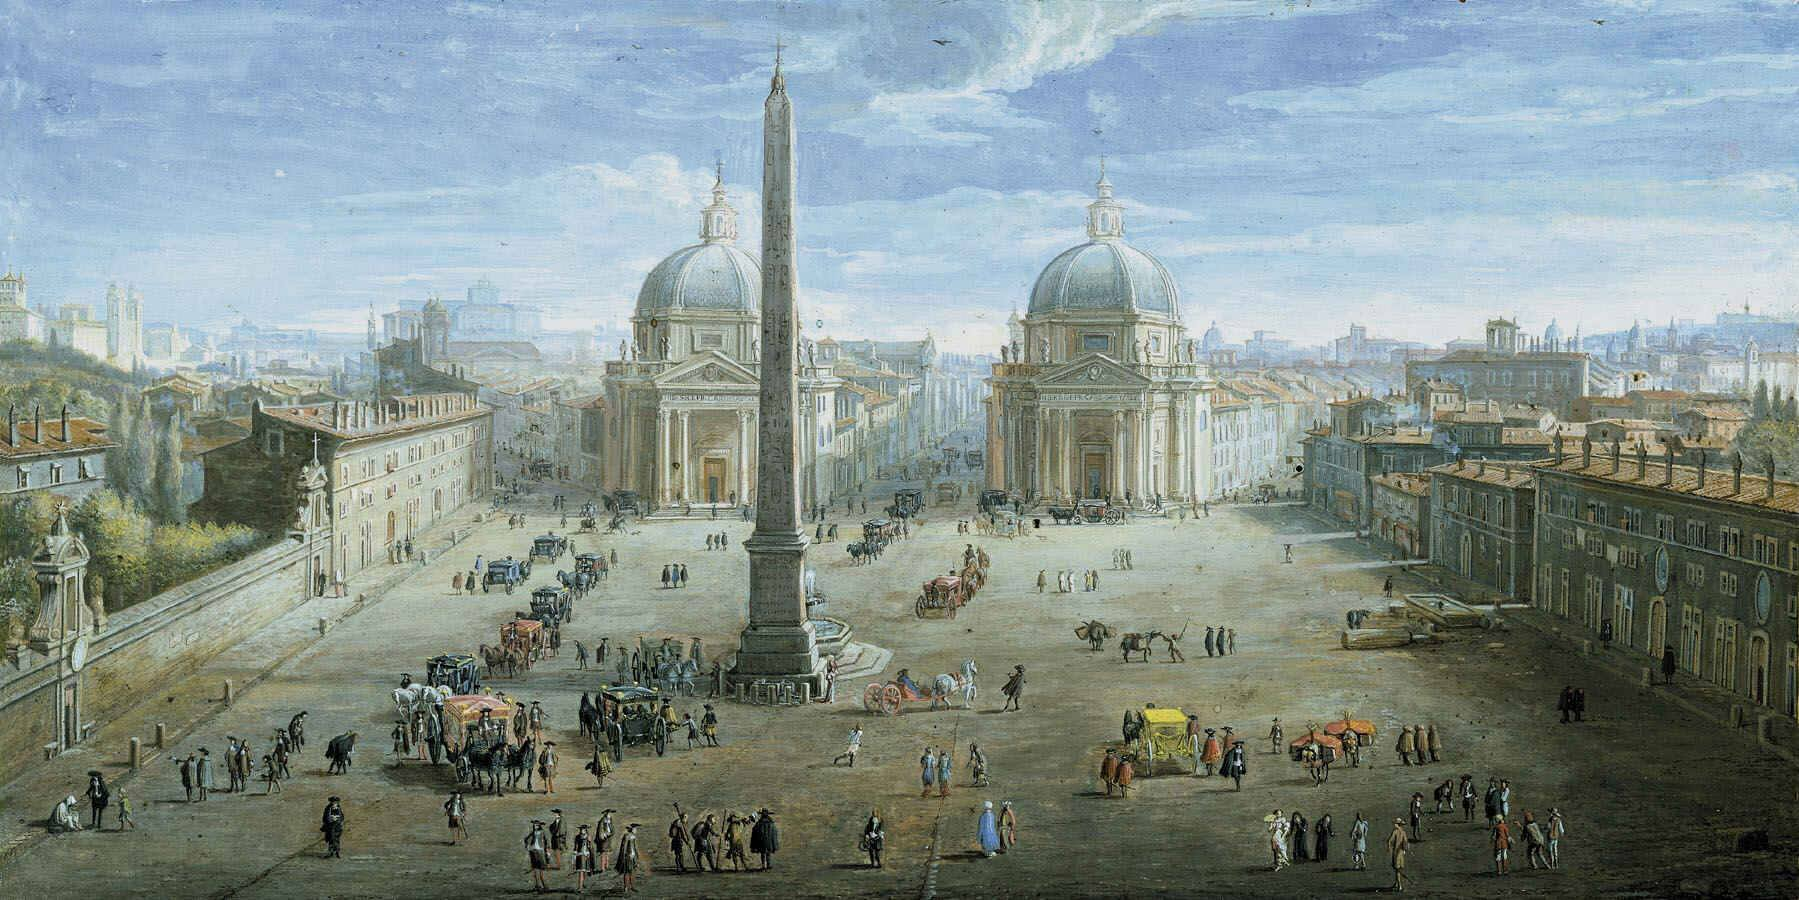
\includegraphics[width=1\textwidth]{/Users/Pancratii/Documents/GitHub/phd/Sections/Projeto_de_Pesquisa_2023-03-18_Teste/Pictures/popolo.jpeg} 
	\captionsetup{labelfont=bf}
	\caption{Vista da \textit{Piazza del Popolo}, em Roma, por Caspar Van Wittel (1652–1736). \textbf{Fonte:} Wikimedia Commons / Sotherby's (coleção privada).}
	\label{fig:popolo}
\end{figure}   

Discorramos rapidamente sobre a ideia de \textit{forma} e traçado. Traçado é o particípio do verbo traçar, \textit{i.e.,} desenhar traços, riscar, sendo o ato ou efeito desse mesmo verbo, resultando, portando, em um 'conjunto de traços', ou, no nosso caso, no 'desenho que representa uma estrutura arquitetônica ou urbanística', o que é equivalente a dizer 'planta', 'projeto', ou, para usar um termo mais antigo, 'traça' (PRIBERAM, TRAÇADO, 2023). Na língua rústica do latim, 'tracto' que dizer 'traçar sulcos', e 'tractus' é a 'delimitação por meio de traços; região, lugar, quarteirão' (FARIA, 1962, p. 1010). Penso que não haja melhor definição que essa: 'delimitação por meio de traços' – que corrobora com a ideia de trajetória de estrada ou mesmo linha férrea (PRIBERAM, TRAÇADO, 2023). \textit{Forma,} porém, é um termo mais complexo.

 \begin{figure}
	\centering
	\includegraphics[width=1\textwidth]{/Users/Pancratii/Documents/GitHub/phd/Sections/Projeto_de_Pesquisa_2023-03-18_Teste/Pictures/nolli_popolo.png}
	\captionsetup{labelfont=bf}
	\caption{\textit{La nuova topografia di Roma} (detalhe), de Gianbattista Nolli (1701-1756), com a \textit{Piazza del Popolo} ao norte. \textbf{Fonte:} UC Berkeley Library.}
	\label{fig:nolli_popolo}
\end{figure} 

\textit{Forma} é a 'configuração das coisas na parte exterior', o que é equivalente a 'feitio' e 'formato' (PRIMERAM, FORMA, 2023). No latim, a coisa complica um pouco, com \textit{'forma'} querendo dizer 'fôrma' (que em português é um 'molde sobre o qual ou dentro do qual se coloca alguma substância fluida, que toma o feitio desse molde'), ou 'todo objeto feito na fôrma'; pode, de fato, ser entendida como 'desenho, modelo, planta', mas também pode ser entendida como 'tipo ideal', ou ainda como 'conformação, configuração, constituição' (FARIA, 1962, p. 407). E, se formos para o campo da filosofia, aí é que a confusão aumenta, pois temos um 'sentido filosófico e particularmente metafísico', um 'sentido lógico', outro 'epistemológico', um metodológico', e, por fim, ainda um 'sentido estético' (MORA, 2001b, p. 1126) – e, portanto, a ideia de \textit{'forma'} escapa-nos neste momento.

Desse modo, na presente pesquisa, meu foco se direciona ao 'traçado urbano' e não à \textit{'forma} urbana'. No entanto, é necessário esclarecer que o termo 'traçado urbano', por sua vez, pode ter mais de uma acepção. Se pensarmos que a \textit{'forma'} da cidade é constituída por seu aspecto tridimensional,\footnote[6]{Aqui faço minhas as palavras de José Lamas (2010, pp. 41 e 48), ao dizer que a forma urbana corresponde "ao meio urbano como arquitectura, ou seja, um conjunto de objectos arquitectónicos ligados entre si por relações espaciais" e que é "a materialização no espaço da resposta a um contexto preciso".} com suas edificações e demais estruturas, podemos deduzir que o 'traçado' é a marca deixada no solo por essa \textit{'forma'}. Logo, o 'traçado' da cidade seria o sulco resultante dos limites dos lotes e quarteirões e dos contornos edificados (que, não raro, definem o próprio desenho das vias, por meio da conjunção de fachadas).\footnote[7]{Note-se que, diferente do que atualmente é lugar comum, o que definia o que era ou não a rua, seu limite, seu contorno, seu espaço, era precisamente a fachada da edificação, que imprime essa linha ao mesmo tempo imaginária e real no solo, diferente do que ocorre hoje. Hoje, o lugar comum é aquele de que o que define a via é o meio-fio — ou o limite do lote, que não coincide com a implantação da edificação, com a marca que a mesma deixa sobre o solo. E isso é fruto da desvinculação entre edificação e lote, entre os limites da edificação e os limites do lote. Mas, se olharmos para nosso passado urbano, veremos algo bem diferente. Basta olharmos uma pintura de Caspar Van Wittel da \textit{Piazza Navona} em Roma e veremos como a praça já era muitíssimo bem definida (pelas edificações), mesmo sem qualquer indício de calçamento, e muito menos de meio-fio.} 

No entanto, aqui, pretendo que o termo 'traçado urbano' tome uma ênfase particular. Isso não exclui o sentido aludido acima, posto que tratarei de contornos edificados, lotes e quarteirões ao falar de 'traçado urbano' ao longo desta tese – porém serei específico quando o fizer. Desse modo, a ênfase que quero dar é a de 'traçado urbano' enquanto sinônimo de 'espaço público', tanto na definição de Vitor Oliveira (2016)\footnote[8]{\textit{'The public spaces system of a city includes (...) the open spaces for movement, which we designate, in a simplified way, as streets, (...) [and] also the open spaces for permanence, which we designate as squares and gardens.'} (OLIVEIRA, 2016, p. 17).} quanto, particularmente, na visão de Huimin Ji e Wowo Ding (2021) – que trazem uma releitura contemporânea de Gianbattista Nolli (Figura \ref{fig:nolli_popolo}). Assim, o termo 'traçado urbano' se relaciona com as vias, praças e áreas públicas de edificações – espaços com acesso franqueado ao público. Percursos, nós e polos abertos e fechados, cobertos e descobertos, percorríveis em um único plano contínuo: o plano do solo.\footnote[9]{Podemos chamar esse plano de 'térreo', ainda que ele comporte variações de altitude e inclinação; porém a ideia é a de que esse é o "plano-base" da cidade, a partir do qual se desenvolvem as edificações, para cima ou para baixo.} Por vias podemos tomar percursos como ruas, calçadões, \textit{woonerfs}, escadarias e alamedas e espaços abertos de parques urbanos (excluídos os maciços vegetais), levando em conta a apropriação dos elementos contidos nesses espaços, como ocorre com os canteiros (HANNES, 2016);\footnote[10]{Canteiros que, atualmente, são considerados algo à parte, algo que não é inerente à via, mas que a define e delimita, posto que, para boa parte das prefeituras, o que determina o limite da via não é o \textit{continuum} das fachadas das edificações, senão o limite dos lotes (muros), as guias de meio-fio e os canteiros: elementos definidores da rua que não mais estão destinados a um uso comum.} bem como estacionamentos descobertos, além de rodovias e ferrovias (posto que servem de passagem para pessoas e suas mercadorias e que possuem uma marca sobre o solo que se relaciona com o desenho do restante da cidade). Por praças, podemos entender tanto a clássica praça, espaço aberto de dimensões superiores à da rua, o largo, o \textit{pocket park}, desde que descobertos – exceção feita aos \textit{'annodamenti'} (dos quais se tratará no momento oportuno), que ficam em uma situação ambígua de área pública de edificação e praça. E as áreas públicas de edificações podem ser exemplificadas pelas naves das igrejas, pelas platéias dos teatros e pelos halls, corredores, pátios e praças cobertas dos  edifícios públicos, galerias comerciais, mercados e \textit{shopping centers}.

Dito isso, reforço que: em relação às 'formas' edificadas, conhecemos os motivos da crise atual  – e podemos mesmo ir mais a fundo, entendendo as dinâmicas inerentes aos materiais, à economia, às tendências ditadas de tempos em tempos pelas publicações e sua relação com o design de outras áreas. Temos ideia de como estabelecer um liame com o passado, inclusive com exemplos projetuais – e, quando não (como no caso do Brasil), temos um método para 'ler' as pré-existências edificadas e, a partir delas, deduzir o \textit{tipo} edilício de um território, de modo a ter o balizador para novas edificações. E nisso reside a força da escola italiana de tipomorfologia urbana. Todavia, mais uma vez: se podemos sabemos como obter respostas em relação à \textit{forma} da cidade, o mesmo não se dá em relação ao seu traçado.

\section{O que(?)}
%Um método de projetação de traçados urbanos

Feito o invitatório, faz-se necessário clarificar alguns pontos acerca da tese que ora escrevo. E penso que valha a pena começar tratando por aquilo que ela 'não' é. Ela não é uma tese filosófica, que tratará acerca da beleza ou da feiúra das cidades. Tampouco falará de 'harmonia' de maneira abstrata, algo como a \textit{Divina Proportione}. Ou de \textit{Simetria}, ou de simbolismo, ou mesmo de pinturicidade e legibilidade das cidades – muito embora meu trabalho termine por incidir tangencialmente sobre esses temas. Ao contrário, minha tese está mais para uma espécie de tratado. E isso mais porque pretendo desenvolver algo feito à mão e sobre algo muito cru, sem muitas abstrações. E não porque darei novas definições para o \textit{universo mundo} da arquitetura (no qual o desenho urbano se insere), posto que aqui pretendo desenvolver um método. Um método? Sim. Mas um método de quê? Um método de como projetar traçados urbanos, e disso trato a seguir.

\section{Por que(?)}
% Problematica

\section{Como(?)}
%Método científico, protocolos, etapas.

\section{Quanto(?)}
%cronogramas (etapa concernente ao projeto de pesquisa)

%28ABR2023 08:55 Aula Codinhoto
	%Minha pesquisa é indutiva, não? Pega indícios (segundo o que tenho visto das aulas do prof. Codinhoto))

\setcounter{secnumdepth}{1}
\chapter{Conceituação}

\section{Sustentabilidade}
%24ABR2023 21:11
%Livro Maretto WAM (descrição correta de unidades de vizinhança, polaridades, sustentabilidade, etc.), link morfologia e sustentabilidade
	%https://books.google.com.br/books?id=t_TDCQAAQBAJ&printsec=frontcover&hl=pt-BR#v=onepage&q&f=false
	%https://books.google.com.br/books?id=Y_ugDgAAQBAJ&printsec=frontcover&hl=pt-BR#v=onepage&q&f=false
% Artigo Maretto sobre Muratori: link entre MURATORI e a ESCOLA ITALIANA com a SUSTENTABILIDADE (não só ambiental, mas projetual como um todo: ambiental, social, econômica, etc.)

%25ABR2023 01:02 Procurando uma ligação entre Unwin e a escola italiana de morfologia urbana, deparei-me com um link na obra de Saverio Muratori, sobretudo em seus projetos urbanos. A saber: por mais que não bebam da mesma fonte Unwin e Muratori se assemelham por suas diretrizes projetuais, sobretudo se observadas à luz dos atuais princípios de sustentabilidade e de exemplos projetuais que se concretizaram "successfully", como Slusehølmen, Skarvet, Expo 98, Quartiere Quinto, entre outros.

\section{Morfologia urbana}
%24ABR2023 21:09
%Artigo Maretto (corrigir artigo na tese, com base no livro)
	%Anotação para Renato: "Estou com muitas coisas na cabeça depois de reler esse artigo.
		%1. Realmente Muratori estava à frente do seu tempo (veja-se a questão de serviços públicos como até centros para idosos em unidades de vizinhança e o aspecto da sustentabilidade, com a vinculação dos terraceamentos, topografia e arborização);
		%2. Só agora me dei conta de que o projeto dos estuários I e II são praticamente o que temos hoje no Slusehølmen em Copenhagen,  e na Expo 98 de Lisboa;
		%3 e mais importante: é IMPRESSIONANTE a semelhança do raciocínio dele com os princípios de Unwin!
		%Renato, você é um gênio! Finalmente achei um link que una ambos! Obrigado."

%Fica apenas um gap por hora: os bairros de Muratori eram restritos, enquanto eu estou pensando numa \textit{urbs}, numa cidade que se expande, numa metrópole, pois é a escala que teremos doravante (ou ao menos de algo que sirva do pequeno assentamento à metrópole a partir da morfologia do sítio).

%25ABR2023 01:50 Há uma questão de escala aqui. Uma cidade Muratoriana (como as Barene di San Giuliano) muitas vezes, para nós, não passam mais do que bairros. A cidade é muito maior.

%01MAI2023 11:28
	%Se observarmos os projetos de Unwin para Letchworth e Hampstead, veremos pouca ou menor consideração pelo relevo do que por um traçado curvilíneo olhado desde cima – o que pode gerar perspectivas, mas que não é necessariamente vinculado à topografia e a todas as suas variáveis e consequências (como caminhabilidade, etc.). Já Muratori leva a morfologia do sítio com afinco em seus projetos, ainda que estes apresentem, diferente de Unwin, conjuntos edificados retilíneos (ao invés de lotes em vias curvas). Não chegam a ser tese e antítese, mas são dissonâncias que podem ser harmonizadas. Logo, o ponto será fazer lotes em vias curvas geradas a partir da topografia (bem como tratar dos edifícios vinculados a ela – ao menos os principais edifícios).
	
	\subsection{Espaço público e privado}
	%18JUN2023 05:29
	Quando falo em 'espaço público' (open space), estou me referindo ao espaço público, semi-público ou privativo com acesso ao público, de ruas e praças ao interior de igrejas. teatros e shoppings centers. Seriam uma espécie de "vão servente" da cidade (se fizermos o paralelo com a classificação entre vãos serventes e servidos própria da escola italiana de tipomorfologia). Já o 'espaço privado' é o equivalente ao "vão servido", ou seja, o vão que só pode ser acessado por meio de um vão servente: do interior das lojas e supermercados ao interior das casas. Meu entendendimento, portanto, não parte de um ponto jurídico e positivista do que é o espaço público ou privado – ou seja, de 'propriedade' pública ou privada segundo tal ou qual lei presentemente em voga. Ao contrário, minha acepção parte de um ponto de vista morfológico, relacionado à possibilidade real de acesso/ingresso a esse espaço, que redunda na sua morfologia, em sua forma, em sua abertura para espaços cada vez mais amplos e acessíveis (topologicamente falando). Exemplo? A nave de uma igreja que se abre para a rua; a praça de alimentação de um shopping center que se conecta a 'ruas' internas à edificação (corredores), chegando finalmente à rua externa; o pátio de um paço público. Todos esses são extensões do espaço público. Espaços públicos (abertos ou cobertos) cujo acesso é franqueado indiscriminadamente à população (mesmo considerando possíveis distorções como a acepção de pessoas em determinador ambientes e horários, posto que, em princípio, o espaço é feito para ser acessado por todos – tanto os que precisam do aspecto apologético da igreja, tanto quanto os que precisam do 'capitalismo' consumista do shopping center).
	
	\textit{Open Spaces} (PATTACINI, 2021)
	
\section{Estruturas naturais: cumeadas, talvegues, linhas de encosta (ou meia pendência)}
\section{Estruturas antrópicas: percursos, nós, polos e tecidos}
%18JUN2023 04:07 Faz mais de uma ou duas semanas que estou enrolado com esses conceitos, sobretudo com a distinção entre nós, nodalidades, polos e polaridades, que parece ser ambígua entre open spaces e edilícia. Ontem discutíamos eu, Luiz e Luca sobre isso e fiz diversas anotações pertinentes no caderno, chegando ao método. O método tenho já relativamente delineado (ao menos em princípio). Falta lapidar esses conceitos e o próprio método em si.) 
	%Para as estruturas naturais, recordo da Maria Rosália Guerreiro – e penso que a Teresa Marat-Mendes tenha algo, assim como o Ian McHarg, não? Isso sem falar nos próprios Caniggia e Maffei e Carlotti (mas, no caso desses três últimos, penso que a coisa se refira mais a __como__ aproveitar essas estruturas naturais).
	% Já para as estruturas antrópicas, não posso senão falar exaustivamente de Caniggia e Maffei, Carlotti e Maretto (e mesmo do artigo que traduzi com o Renato).
%18JUN2023 04:31 Observando o mapa do território de São Paulo e do Paraná com as cumeadas, bacias e ferrovia Sorocabana (que desenvolvi na dissertação, p. 59), é interessante notar que o rio Paraná será um polo final para a cumeada que atravessa o território da CTNP (faltando apenas definir onde seria o polo inicial); para a ferrovia, poderíamos adotar a travessia do rio Tibagi como primeiro nó, terminando no rio Ivaí (ou talvez em Cianorte); porém, se observarmos a conjunção dos dois fatores e a estruturação (parcelamento) do território, podemos – realmente – pensar em Londrina e Maringá como duas polaridades territoriais, posto que é nesses dois polos (nessas duas cidades) que ocorre uma "inflexão", uma mudança: a saber, a ferrovia deixa de subir o relevo para passar a se assentar sobre o traçado da cumeada territorial, dando origem a um território único (unitário).

\chapter{Uma análise de Unwin}

Iniciemos pelo sumário da obra de Raymond Unwin. Após o prefácio temos os seguintes capítulos:
\begin{enumerate}
	\item \textit{Of Civic Art as the Expression of Civic Life};
	\item \textit{Of the Individuality of Towns, with a Slight Sketch of the Ancient Art of Town Planning};
	\item \textit{Of Formal and Informal Beauty};
	\item \textit{Of the City Survey};
	\item \textit{Of Boundaries and Approaches};
	\item \textit{Of Centres and Enclosed Places};
	\item \textit{Of the Arrangement of Main Roads, their Treatment and Planting};
	\item \textit{Of Site Planning and Residential Roads};
	\item \textit{Of Plots and the Spacing and Placing of Buildings and Fences};
	\item \textit{Of Buildings, and how the variety of Each must be dominated by the Harmony of the Whole};
	\item \textit{Of Co-operation in Site Planning, and how Common Enjoyment benefits the Individual};
	\item \textit{Of Building Bye-laws}.
	\end{enumerate}
	
\chapter{Modus faciendi atual}
%10JUN2023 17:52 CASA
%Em que vamos agir, incidir, senão sobre o \textit{modus faciendi} atual? (Isso faz da minha pesquisa uma DSR, na qual busco incrementar ou aperfeiçoar um método existente? Ou não?). Ora, e o que é esse modus faciendi atual? Ou melhor, como se projetam loteamentos e novas áreas urbanas atualmente? Onde posso descobrir isso? – Mascaró e outros autores podem me ajudar. A grande questão é descobrir de onde Mascaró tirou suas fontes (a não se que seja tudo empírico) e que livros, no Brasil e no exterior, ensinam como projetar traçados urbanos, de modo a entender sua lógica e como ela pode ser 'capovolta'.)

\chapter{Variações sobre um tema: o processo de projeto de um novo traçado urbano em diversos cenários}

Como costumo trabalhar ouvindo música, é natural que termine por projetar seguindo um pouco da lógica dos compositores que ouço, ou ao menos da estrutura impressa em suas composições. %(da lógica impressa na estrutura de suas composições).
Logo, não me posso furtar da analogia entre arquitetura e música. Não daquela analogia entre proporções, como existe entre ordens arquitetônicas, escala musical e proporções matemáticas – essa deixo para aqueles que são mais pitagóricos, mais platônicos do que eu; ou ao menos para aqueles mais versados nesse tema. Ao contrário, minha analogia se dá na estruturação, da lógica compositiva. A analogia entre o processo de projeto e o processo de composição, entre o traçado e sua configuração impressa no solo e a estrutura musical (nas formas em que veremos a seguir, como variações sobre um tema, forma cíclica, etc.).

Aqui, as estruturas naturais serão meu "tema" e o traçado urbano o ulterior "desenvolvimento" desse "tema".

%27ABR2023 14:17 Ainda sobre o artigo do Maretto sobre Muratori.
	%Note-se que Muratori projetava com percursos principais, secundários, unidades de vizinhança, edificações baseadas no tipo, etc. Ora, diante disso, que contribuição inovadora eu posso dar? O método já está todo ali. Bom, algo está ligado à questão de escala. Muratori fazia apenas pequenas cidades (que até poderiam se expandir, mas que eram estanques em si mesmas enquanto projetos), enquanto hoje temos metrópoles, que seriam (em termos de escala) iguais a uma somatória de diversas dessas cidades, o que me faz pensar em projetar conforme Muratori, mas sempre pensando no meu framework de maior escala de modo a formar um grande quadro urbano a partir de pequenas cidades muratorianas (o que, para mim, ou para o próprio Unwin e Vieira, seriam bairros) – há que se ver o que Muratori entende como "cidade" (é apenas morfológico? Depende de quais polaridades? Quais equipamentos?). Além disso, há uma outra questão, não apenas de escala, mas de logística e temporalidade, i. e., Muratori projetava os edifícios prontos – o que é diferente da nossa realidade – e cidades que eram pequenas (pequenas unidades, como já mencionei), porém, como são as unidades de terra, os lotes? Cada quadra seria já um lote? Isso funciona talvez numa Expo '98, mas será se funciona no Brasil. Posso abrir os percursos conforme o relevo e fazer um Skarvet da vida, com uma quadra-lote, ou talvez um Slusehølmen da vida, com um grande quarteirão que deixa um espaço aberto interno (enquanto os apartamentos constituiríam os lotes). Talvez. Mas isso é possível? É factível? Sim e sim. Mas é viável? Isso já não sei (e que o diga Goiânia). Isso sem mencionar que a nossa lógica é aquela lógica lusa em que temos ruas com lotes e quintais e que nossas unidades de vizinhança (muratorianas) se dão mais pela praça pública do que por uma espécie de praça semi-pública (como no mundo anglo-saxão) – embora tivéssemos os cortiços e paços. Desse modo, preciso pensar em projetar numa escala maior que a cidade muratoriana e de tal modo que o traçado incorpore os lotes de modo a direcionar, talvez, o formato dos edifícios, mas sem necessariamente os determinar (como o faria Muratori), de modo a tornar viável em escala, espaço, logística e tempo.
		%% 27ABR2023 15:18 No caso da escala e dos projetos de pequenas cidades integradas entre si formando um conjunto, isso poderia entrar como cunhas verdes, cidades-satélites, cidade-região ou algo assim?

\chapter{Método}
\section{Passo-a-passo}

\chapter*{Anexos}
\addcontentsline{toc}{chapter}{Anexos}

\section*{Descrição dos procedimentos efetuados, algoritmos e códigos}
%\addcontentsline{toc}{section}{Descrição dos procedimentos efetuados, algoritmos e códigos}


\end{document}          
